\chapter{Assignment: Data Preprocessing}
\label{ch:arheo_data_preprocessing}

\newthought{Data preprocessing is crucial in archeology.} The data often contains many diverse labels, some of which are certain and others speculative. Machine learning doesn't handle categorical data with many different labels well, hence we need to preprocess the data.

We will use the \href{https://archaeologydataservice.ac.uk/catalogue/adsdata/arch-1115-2/dissemination/csv/pottery/pottery.csv}{pottery} data from the Antikythera data base. The data contains 13,865 data instances and 36 features describing the pottery collected across the full extent of the Greek island of Antikythera.

Let us look at the VesselPart feature, which describes the part of the ceramic vessel involved and it has 34 values.

\begin{figure*}[h]
    \centering
    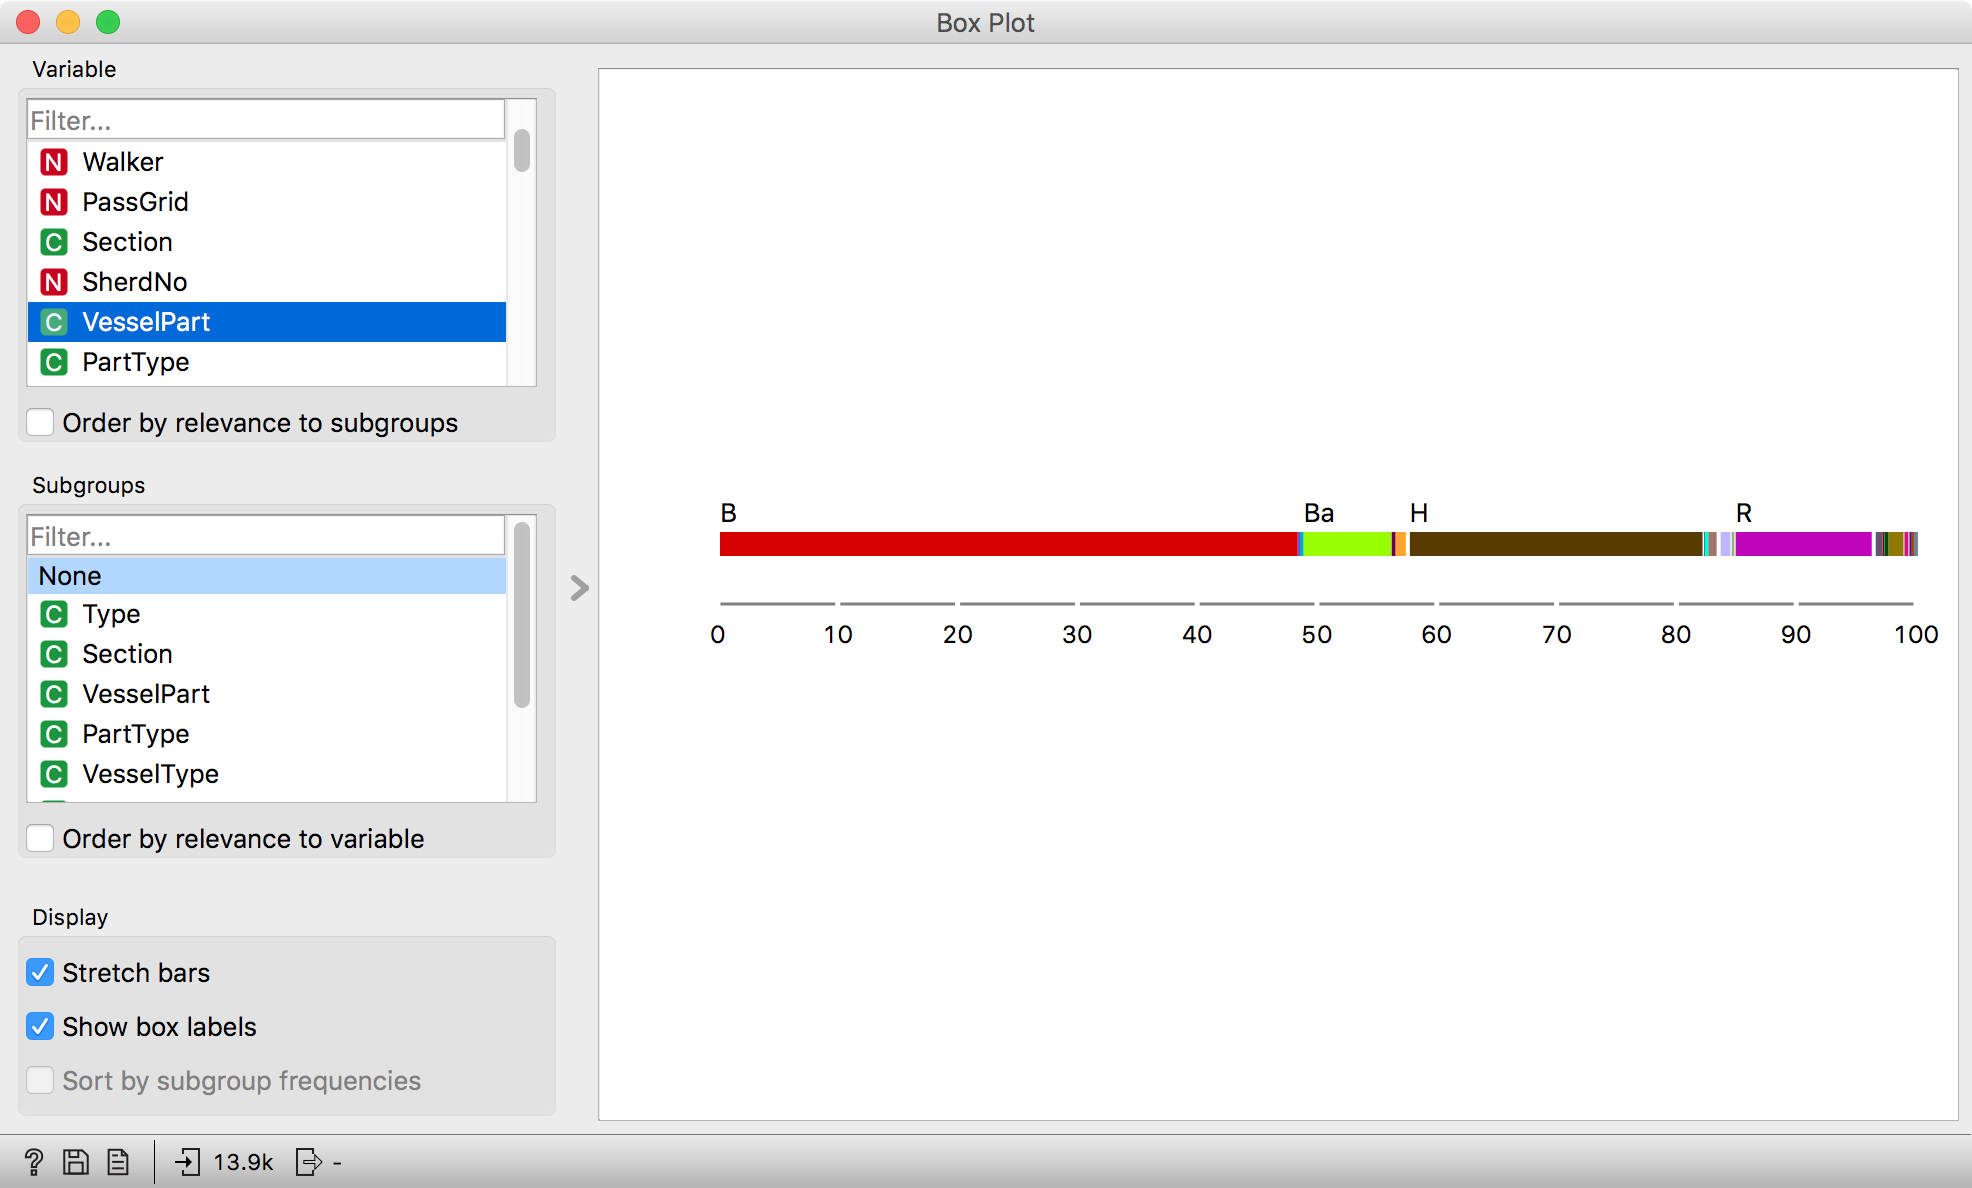
\includegraphics[scale=0.35]{box-plot-vesselpart.png}
    \caption{$\;$} % empty caption for proper page setting
\end{figure*}

But looking at the \widget{Box Plot}, we notice there are 4 fairly frequent values, while others are rare. We would like to keep B (body), Ba (base), H (handle), and R (rim), and consider all the others as one group.

\begin{figure*}[h]
    \centering
    \newcommand{\before}{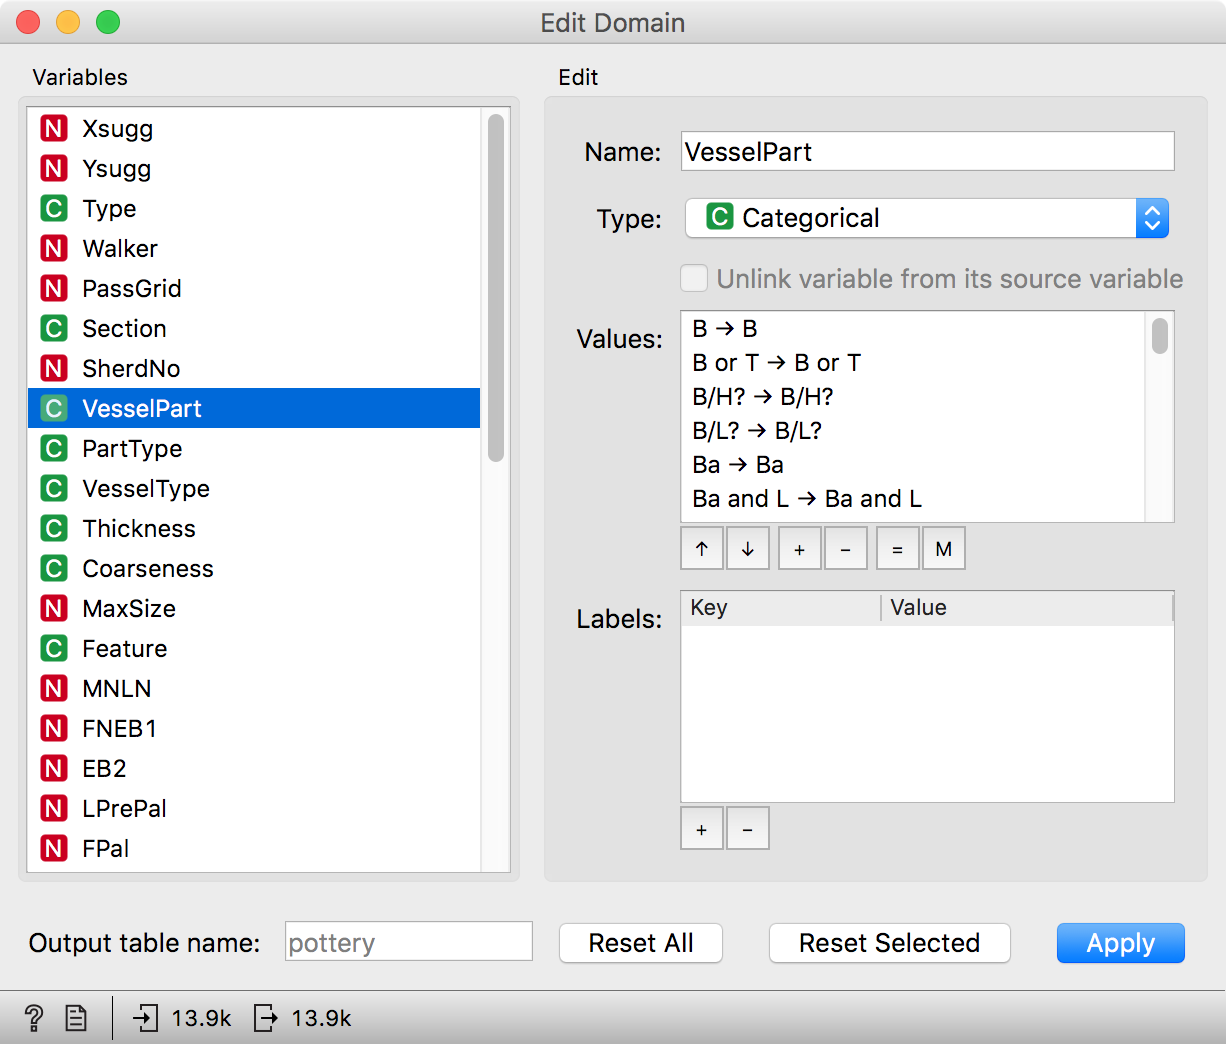
\includegraphics[scale=0.35]{edit-domain-before.png}}
    \newcommand{\after}{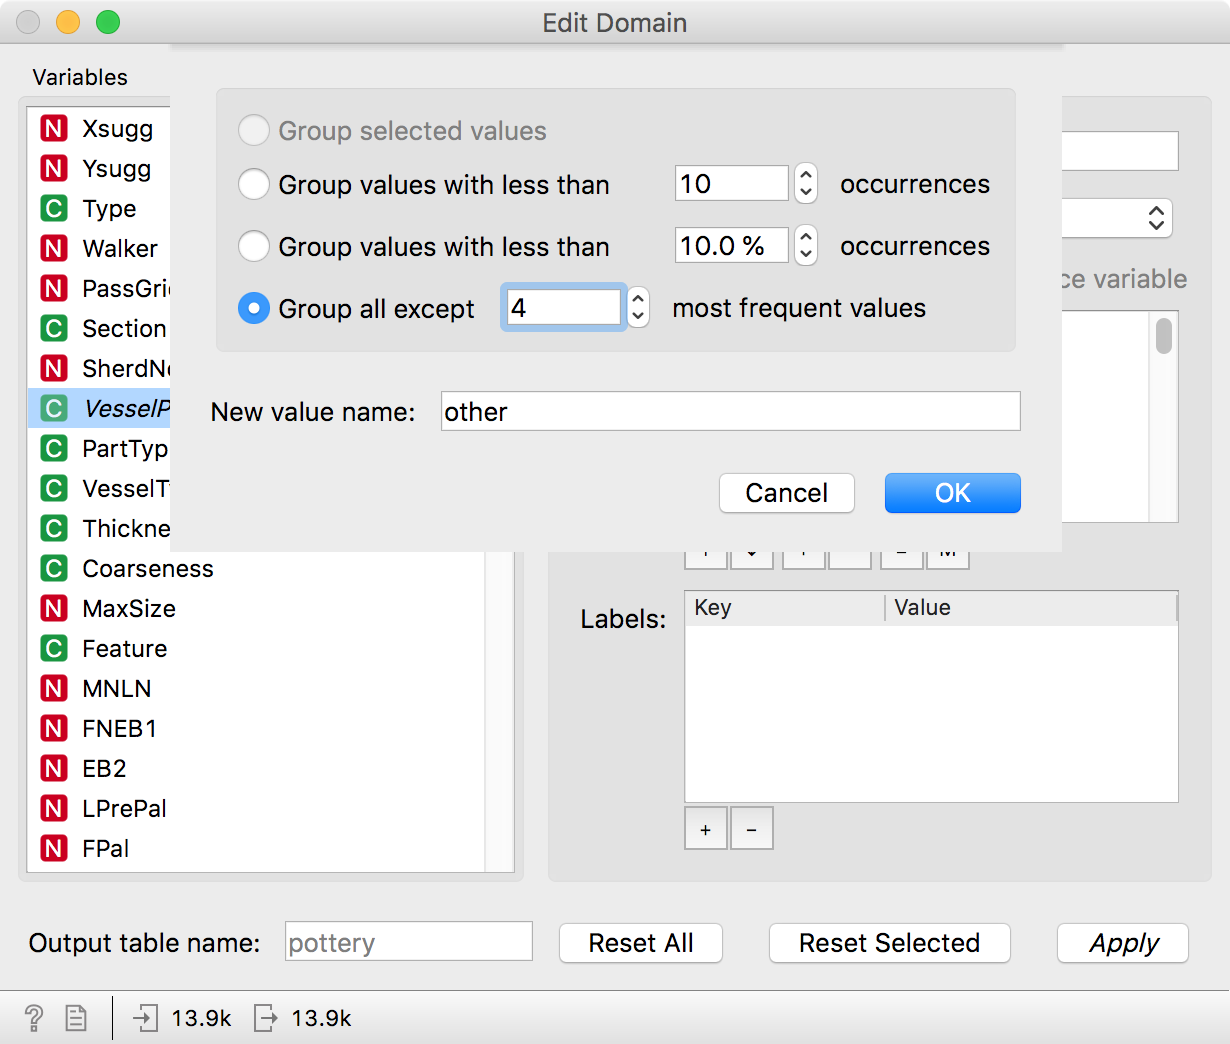
\includegraphics[scale=0.35]{edit-domain-during.png}}
    \infinitewidthbox{
    \stackinset{r}{-0.5\linewidth}{t}{0.0\linewidth}{\after}{\before}\hspace{8cm}
    }
\end{figure*}

We will use \widget{Edit Domain} to merge infrequent values together. Select \textit{VesselPart} and press M. This opens a dialogue for merging values. You can use any technique you wish. Here, since we know there are 4 frequent values, we will use the final option, \textit{Group all except 4 most frequent values}. We can also give the name to the new value, but let's leave it a \textit{other} for now.

\newpage

You can see the less frequent values have been remapped. Do not forget to press \textit{Apply} once you have finished editing. Looking at the Box Plot, the values are now much easier to interpret.

\begin{marginfigure}
    \centering
    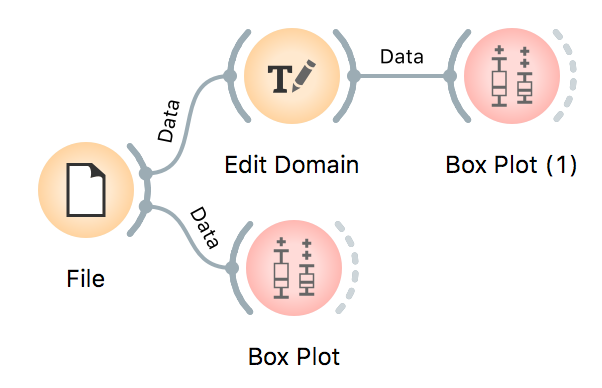
\includegraphics[scale=0.5]{workflow.png}
\end{marginfigure}

\begin{figure}[h]
    \centering
    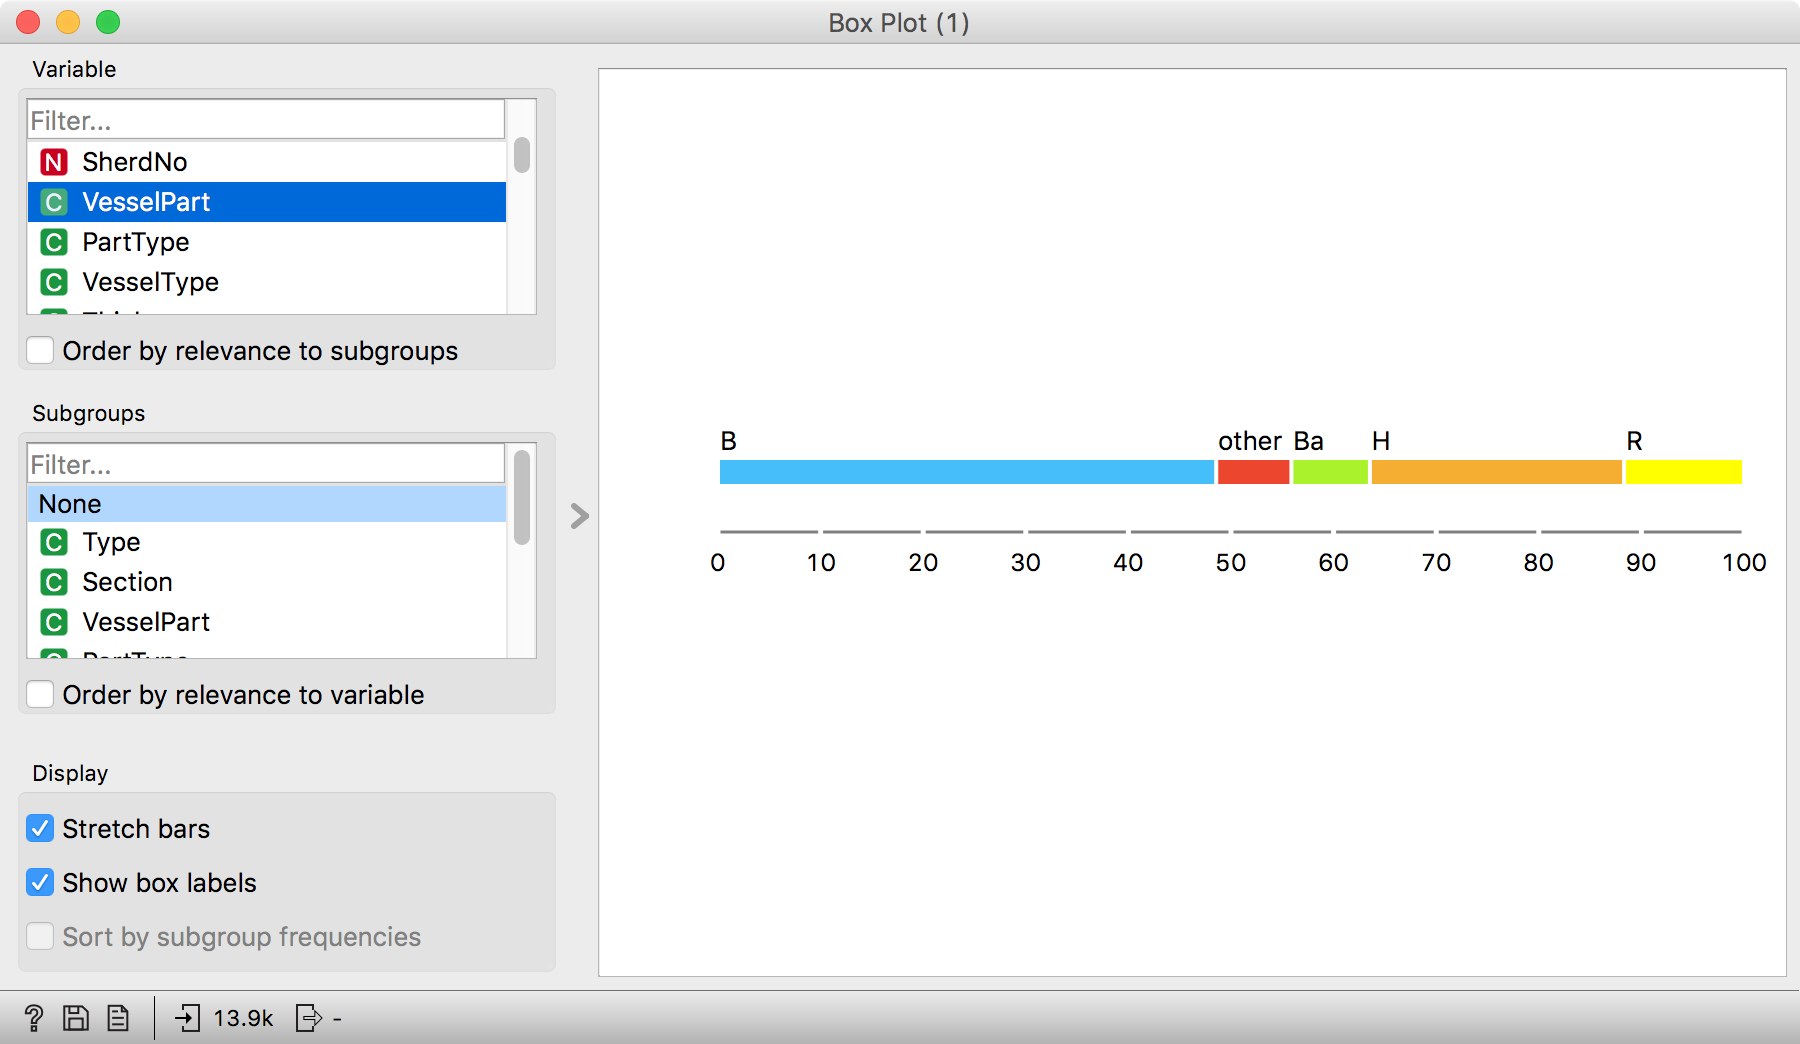
\includegraphics[scale=0.35]{box-plot-after.png}
    \caption{$\;$} % empty caption for proper page setting
\end{figure}

\subsection{Assignment}

Preprocess the pottery data using the technique from above and answer the following questions:
\begin{itemize}
    \item Put metadata to meta attributes using Select Columns. Which features did you put there? Why?
    \item Which features had to be preprocessed by merging infrequent values?
    \item Is there another way we could merge values?
    \item Use Box Plot after Edit Domain and 
\end{itemize}
